\documentclass{beamer}
\usetheme{metropolis}

\usepackage{marvosym}
\usepackage{tikz}
\usetikzlibrary{positioning}

\setbeamertemplate{itemize item}{\scriptsize\raise1.25pt\hbox{\donotcoloroutermaths$\bullet$}}
\setbeamertemplate{itemize subitem}{\tiny\raise1.5pt\hbox{\donotcoloroutermaths$\blacktriangleright$}}
\setbeamertemplate{itemize subsubitem}{\tiny\raise1.5pt\hbox{\donotcoloroutermaths\Smiley}}
\setbeamertemplate{enumerate item}{\insertenumlabel.}
\setbeamertemplate{enumerate subitem}{\insertenumlabel.\insertsubenumlabel}
\setbeamertemplate{enumerate subsubitem}{\insertenumlabel.\insertsubenumlabel.\insertsubsubenumlabel}
\setbeamertemplate{enumerate mini template}{\insertenumlabel}

\title{%
  Discrete Channels w/Noise \\
  \normalsize A Mathematical Theory of Communication, Part II}
\author{David Sanders}

\begin{document}

  \maketitle

  \section{First, some review... \\
           \small (p.1 -- 19 of Shannon)}

  \begin{frame}{Introduction \small (p.1)}
    \begin{itemize}
      \item Context of signal processing (PCM, PPM)
      \item Communication is reproducing messages sent over channels
      \item Mathematical theory shouldn't care about meaning
      \begin{itemize}
        \item Instead, focus on message as one selected from many possibilities
        \item Absence of meaning allows message to be viewed as random variable
      \end{itemize}
      \item Any monotonic, increasing function of number of possibilities $n$
      is measure of information
      \begin{itemize}
        \item Use $\log n$
        \begin{itemize}
          \item Engineering parameters vary linearly w/log of possibilities
          \item More intuitive -- 2 disks have twice the information ($(2^x)(2^x) = 2^{2x}$ states)
          \item Mathematically convenient -- ``downgrades" operations; $\log ab
          = \log a + \log b$, $\log x^a = a \log x$, etc.
        \end{itemize}
      \end{itemize}
    \end{itemize}
  \end{frame}

  \begin{frame}{Introduction \small (p.2)}
    \begin{figure}
      \centering
      \includegraphics[scale=0.5]{images/basic.png}
      \caption{A general communications system.}
    \end{figure}
  \end{frame}

  \begin{frame}{Discrete Noiseless Channel \small (p.3)}
    The capacity $C$ of a discrete noiseless channel in bits per second:
    \begin{equation}
      C = \lim_{T \rightarrow \infty} \frac{\log N(T)}{T}
    \end{equation}
    where $N(T)$ is the number of allowed message of a given length $T$:
    \begin{equation}
      N(t) = N(t - t_1) + N(t - t_2) + \cdots + N(t - t_n)
    \end{equation}
  \end{frame}

  \begin{frame}{Discrete Source of Information \small (p.5)}
    Kinds of sources:
    \begin{itemize}
      \item Nth-order approximations:
      \begin{itemize}
        \item Zero-order: independent and equiprobable
        \item First-order: independent but with frequencies from some text
        \item Second-order: dependency on previous symbol
        \item etc.
      \end{itemize}
      \item Markov processes: Finite number of states with transition probabilities.
      \begin{itemize}
        \item Ergodic processes: Statistical properties approach definite
          limits as the length of sequences become longer.
      \end{itemize}
    \end{itemize}
  \end{frame}

  \begin{frame}{Entropy Properties \small (p.10)}
    Chosen measure of information $H(p_1, p_2, \ldots, p_n)$ must have these
    properties:
    \begin{enumerate}
      \item $H$ should be continuous over any $p_i$.
      \item If all $p_i = \frac{1}{n}$, then $H$ should be monotonically
        increasing function of $n$.
      \item If choice broken into successive choices, then should be weighted
        sum of choices.  Example:
        \begin{equation}
          H\left(\frac{1}{2}, \frac{1}{3}, \frac{1}{6}\right) = H\left(\frac{1}{2},
          \frac{1}{2}\right) + \frac{1}{2} H\left(\frac{2}{3}, \frac{1}{3}\right)
        \end{equation}
    \end{enumerate}
  \end{frame}

  \begin{frame}{Entropy Properties \small (p.10)}
    From the previous properties, we get this:
    \begin{equation}
      H(p_1, p_2, \ldots, p_n) = \sum_i p_i \log \frac{1}{p_i} = -\sum_i p_i \log p_i
    \end{equation}
  \end{frame}

  \begin{frame}{Joint and Conditional Entropy \small (p.12)}
    For two events $x$ and $y$, the joint entropy is:
    \begin{equation}
      H(x, y) = -\sum_{i,j} p(i,j) \log p(i,j)
    \end{equation}
    while
    \begin{align}
      H(x) &= -\sum_{i,j} p(i,j) \log \sum_k p(i,k) \\
      H(y) &= -\sum_{i,j} p(i,j) \log \sum_k p(k,j)
    \end{align}
  \end{frame}

  \begin{frame}{Joint and Conditional Entropy \small (p.12)}
    Conditional probability is:
    \begin{equation}
      p_i(j) = \frac{p(i,j)}{\sum_k p(i,k)}
    \end{equation}
    Conditional entropy is:
    \begin{equation}
      H_x(y) = -\sum_{i,j} p(i,j) \log p_i(j)
    \end{equation}
    Based on all these definitions, we get:
    \begin{equation}
      H(x,y) = H(x) + H_x(y)
    \end{equation}
  \end{frame}

  \section{Discrete Noisy Channels \\
           \small (p.19 -- 28 of Shannon)}

  \begin{frame}{Basic Concepts \small (p.19)}
    What is noise ($N$)?
    \begin{itemize}
      \item Perturbation of transmitted signal ($S$) at either terminal or in
      channel
      \item Received signal ($E$) may not be same as transmitted signal ($S$)
    \end{itemize}

    \begin{figure}
      \footnotesize
      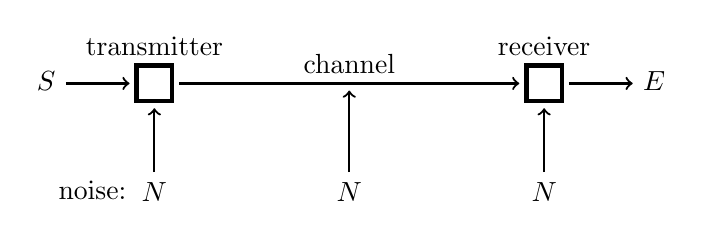
\begin{tikzpicture}[scale=0.45,->,thick]
        \draw (-2,0.5) -- (-0.2,0.5);
        \node [left] at (-2,0.575) {$S$};
        \node [below left] at (0,-1.95) {noise:};

        \draw (0.5,-2) -- (0.5,-0.2);
        \node [below] at (0.5,-2) {$N$};

        \draw [ultra thick] (0,0) rectangle (1,1);
        \node [above] at (0.5,1) {transmitter};

        \draw (1.2,0.5) -- (10.8,0.5);
        \node [above] at (6,0.5) {channel};

        \draw (6,-2) -- (6,0.3);
        \node [below] at (6,-2) {$N$};

        \draw [ultra thick] (11,0) rectangle (12,1);
        \node [above] at (11.5,1) {receiver};

        \draw (11.5,-2) -- (11.5,-0.2);
        \node [below] at (11.5,-2) {$N$};

        \draw (12.2,0.5) -- (14,0.5);
        \node [right] at (14,0.575) {$E$};
      \end{tikzpicture}
      \caption{Sources of noise.}
    \end{figure}
  \end{frame}

  \begin{frame}{Kinds of Noise \small (p.19)}
    Two different kinds of noise:
    \begin{itemize}
      \item Distortion: $E \neq S$ and $E = f(S)$
      \begin{itemize}
        \item If $f^{-1}$ exists for $f$, recovery of $S$ from $E$ is possible
      \end{itemize}
      \item Random noise: $E \neq S$ and $E = f(S, N)$
      \begin{itemize}
        \item Noise $N$ is random variable; may be represented by stochastic
        process
      \end{itemize}
    \end{itemize}
  \end{frame}

  \begin{frame}{Generalization \small (p.19)}
    Generalization via finite-state, noise-free channel:
    \begin{equation}
    p_{\alpha,i}(\beta,j)
    \end{equation}
    Probability, if channel in state $\alpha$ and symbol $i$ transmitted, that
    symbol $j$ received and channel left in state $\beta$.

    If symbols independently perturbed by noise, channel state omitted (only
    one state):
    \begin{equation}
    p_{i}(j)
    \end{equation}
    Probability, if symbol $i$ transmitted, that symbol $j$ received.
  \end{frame}

  \begin{frame}{Different Entropies \small (p.19)}
    In noisy channel, two statistical processes:
    \begin{itemize}
      \item Source
      \item Noise
    \end{itemize}
    Therefore, a number of different entropies are considered:
    \begin{itemize}
      {\small
        \item $H(x)$ -- entropy of transmitted signal
        \item $H(y)$ -- entropy of received signal
        \item $H(x,y)$ -- joint entropy of transmitted and received signals
        \item $H_x(y)$ -- entropy of received signal when transmitted signal is known
        \item $H_y(x)$ -- entropy of transmitted signal when received signal is known
      }
    \end{itemize}
  \end{frame}

  \begin{frame}{Relationship of Entropies \small (p.19)}
    Relationship of previous entropies given below:
    \begin{equation}
      H(x,y) = H(x) + H_x(y) = H(y) + H_y(x)
    \end{equation}
    More descriptively,
    \begin{itemize}
      \item $H(x,y) = H(x) + H_x(y)$ -- joint entropy is entropy of $x$ plus
      entropy of $y$ not accounted for by $x$
      \item $H(x,y) = H(y) + H_y(x)$ -- joint entropy is entropy of $y$ plus
      entropy of $x$ not accounted for by $y$
    \end{itemize}
    With no noise,
    \begin{itemize}
      \item $H(x,y) = H(x)$ and $H_x(y) = 0$
      \item Or, $H(x,y) = H(y)$ and $H_y(x) = 0$
    \end{itemize}
  \end{frame}

  \begin{frame}{An Example \small (p.20)}
    An example,
    \begin{itemize}
      \item Symbols $0$ and $1$
      \item Probabilities $p_0 = p_1 = \frac{1}{2}$
      \item $1000$ symbols per second
      \item $\implies$ $1000$ bits per second
    \end{itemize}
    If noise causes $1$ in $100$ symbols ($1\%$) to be received incorrectly,
    what is overall rate of transmission?
    \begin{itemize}
      \item Definitely $< 1000$ bits per second
      \item $1000 \times 0.01 = 990$ bits per second?
    \end{itemize}
  \end{frame}

  \begin{frame}{An Example \small (p.20)}
    If rate of transmission is $1000 \times 0.01 = 990$ bits per second, then
    error rate of $50\%$ would still permit transmission of $500$ bits per
    second even though message is completely unintelligible.  So this is
    clearly not the answer.  Then what is?
  \end{frame}

  \begin{frame}{An Example \small (p.20)}
    Must subtract from transmitted information $H(x)$ the portion of $H(x)$
    missing in received information $H(y)$.  Alternatively, the uncertainty in
    the transmitted information $H(x)$ given that we know the received signal
    $y$:
    \begin{equation}
      R = H(x) - H_y(x)
    \end{equation}
    $R$ is the actual rate of transmission.  $H_y(x)$ is the
    \emph{equivocation} (average ambiguity of received signal).
  \end{frame}

  \begin{frame}{An Example \small (p.20)}
    Given received signal, two possible outcomes regarding transmitted signal:
    \begin{itemize}
      \item Correct symbol was received with probability $p_{correct}$
      \item Incorrect symbol was received with probability $p_{incorrect}$
    \end{itemize}
  \end{frame}

  \begin{frame}{An Example \small (p.20)}
    In previous example,
    \begin{itemize}
      \item $p_{correct} = 0.99$ and $p_{incorrect} = 0.01$
      \item $H_y(x) = -\left[ 0.99 \log 0.99 + 0.01 \log 0.01 \right] \approx 0.081$ bits per symbol
      \item $R \approx 1000 - 81 = 919$ bits per second
    \end{itemize}
    If $p_{correct} = p_{incorrect} = \frac{1}{2}$,
    \begin{itemize}
      \item $H_y(x) = -\left[ 0.5 \log 0.5 + 0.5 \log 0.5 \right] = 1$ bits per symbol
      \item $R = 1000 - 1000 = 0$ bits per second
    \end{itemize}
  \end{frame}

  \begin{frame}{Correction Theorem \small (p.20--21)}
    \textbf{Correction Theorem} {\footnotesize (Theorem 10 from Shannon)}: \\
    (Part I) If correction channel has capacity $H_y(x)$, possible to send correction
    data to correct all but arbitrarily small faction $\epsilon$ of errors. \\
    (Part II) Not possible if channel has capacity less than $H_y(x)$.
  \end{frame}

  \begin{frame}{Correction Theorem \small (p.21)}
    \textbf{Proof of part I}: \\
    For sequences of transmitted signals $M$ and received signals $M'$, there
    are $T H_y(x)$ of the $M$'s which could have produced each $M'$.
    Therefore, $T H_y(x)$ binary digits of correction data to send every $T$
    seconds.
  \end{frame}

  \begin{frame}{Correction Theorem \small (p.21)}
    \textbf{Proof of part II}: \\
    For any discrete variables $x$, $y$, and $z$:
    \begin{align}
      H_y(x, z) &\ge H_y(x) & \\
      H_y(z) + H_{yz}(x) &\ge H_y(x) & \\
      H_{yz}(x) &\ge H_y(x) - H_y(z) &\; \left( \ge H_y(x) - H(z) \right) \\
      \implies H_{yz}(x) &\ge H_y(x) - H(z) &
    \end{align}
    If $x$ is source, $y$ is received, and $z$ is correction signal, then
    $H_{yz}(x)$ is residual information while knowing transmitted signal and
    correction data.
  \end{frame}

  \begin{frame}{Actual Rate of Transmission \small (p.21--22)}
    Alternative formulations of actual rate of transmission:
    \begin{align}
      R &= H(x) - H_y(x) \\
        &= H(y) - H_x(y) \\
        &= H(x) + H(y) - H(x,y)
    \end{align}
    Equation 19 is information transmitted less ambiguity of received.
    Equation 20 is information received less part due to noise.  Equation 21 is
    number of bits common to $H(x)$ and $H(y)$.
  \end{frame}

  \begin{frame}{Capacity of Noisy Channel \small (p.22)}
    Capacity $C$ of noisy channel:
    \begin{equation}
      C = \max(H(x) - H_y(x))
    \end{equation}
    where max is with respect to all possible information sources.  This
    theorem may seem rather mudane.  But we'll soon why it's interesting.
  \end{frame}

  \begin{frame}{Fundamental Theorem of Noisy Channel \small (p.22)}
    \begin{itemize}
      \item Why talk about capacity of noisy channel?  Can such a channel
        transmit anything but corrupted data?
      \item Redundancy $=$ lower probability of errors
      \item Must redundancy be increased indefinitely to continue reducing
        error rate?  Will channel capacity be entirely used up by redundancy?
      \item No!  Errors can be reduced through proper encoding, which utilizes
        redundancy but does not consume increasingly more capacity.
    \end{itemize}
  \end{frame}

  \begin{frame}{Fundamental Theorem of Noisy Channel \small (p.22)}
    The fundamental theorem of a noisy channel:

    \textit{Let channel have capacity $C$ and source have entropy per second
    $H$.  If $H \le C$, there is coding system such that output of source can
    be transmitted over channel with arbitrarily small frequency of error
    (equivocation).  If $H > C$, possible to encode source so that equivocation
    less than $H - C + \epsilon$.  No encoding method with equivocation less
    than $H - C$.}
  \end{frame}

\end{document}
